\documentclass[12pt,a4paper,twoside,%
BCOR12mm,DIV12,%
headsepline,%
cleardoubleempty,chapterprefix,parskip,%
liststotoc,idxtotoc,bibtotoc]{scrbook}

\usepackage[english, ngerman]{babel}
\usepackage[utf8]{inputenc}
\usepackage[T1]{fontenc}
\usepackage{mathptmx}
\usepackage[scaled=0.92]{helvet}
\usepackage{courier}
\usepackage{amsmath}
\makeatletter
\def\displaymath{\typeout{*** Do not use DISPLAYMATH. Use \[...\] instead ***}}
\def\eqnarray{\typeout{*** Do not use EQNARRAY(*). Use align(*)-environment instead ***}}
\makeatother
\usepackage{amsfonts}
\usepackage{amstext}
\usepackage{subfigure}
\usepackage{color}
\usepackage{graphicx}
\usepackage{ifpdf}
\usepackage{makeidx}
\usepackage{nomencl}
\usepackage{setspace}

% first include hyperref, then cite
\usepackage[plainpages=false,pdfpagelabels]{hyperref}
\usepackage{cite}

\usepackage{lscape}
\usepackage{tabularx}

\ifpdf
    \definecolor{brown}{cmyk}{0, 0.81, 1, 0.60}
    \hypersetup{%
      pdftitle={Secure Program Execution}, %%%% HIER AENDERN!!!
      pdfsubject={Bachelorarbeit},
      pdfauthor={Dorian Eikenberg},           %%%% HIER AENDERN!!!
      pdfkeywords={KEYWORDS},      %%%% HIER AENDERN!!!
      colorlinks=false, urlcolor=blue, citecolor=brown,
      bookmarksnumbered=true,
    }
\else   
\fi

\listfiles

\begin{document}
\onehalfspacing

\frontmatter

\pdfbookmark[0]{Titelseite}{tit}
% Titelseite

\begin{titlepage}
  \centering
  
\includegraphics[width=5cm]{fig/unilogo}\\

  \vfill
  \huge
  Das ist der Titel der Bachelorarbeit\\*[40pt]
  \normalsize

  \vfill
  \large
  Bachelorarbeit\\[0.25em]
  \normalsize
  von\\
  \Large
  VORNAME NACHNAME\\

  \vspace{5mm}
  \normalsize
  aus\\ GEBURTSORT\\[1cm]
  vorgelegt am\\[5mm]
  Lehrstuhl für Rechnernetze und Kommunikationssysteme\\
  Prof.\ Dr.\ Martin Mauve\\ 
  Heinrich-Heine-Universität Düsseldorf\\[0.5cm]
  MONAT JAHR\\[0.5cm]
  Betreuer:\\
  Dipl.\ Wirtsch.-Inf.\ Vorname Nachname\\
  VORNAME NACHNAME M.\,Sc.
    
\end{titlepage}


%%% Local Variables: 
%%% mode: latex
%%% TeX-master: "master"
%%% End: 


\cleardoublepage

\pdfbookmark[0]{Zusammenfassung}{abstract}
\begin{center} 
\huge Zusammenfassung
\end{center}

Hier beschreibe ich nun auf einer Seite, welches Problem ich betrachtet, wie ich es gel\"ost habe
und was die Hauptergebnisse meiner Arbeit sind.



\cleardoublepage

\pdfbookmark[0]{Danksagung}{ack}
\begin{center} 


\huge Acknowledgments

\end{center}
I would like to thank all people who supported me during my work on this thesis.

My special thanks go to Philipp Hagemeister who always provided me with helpful advice.

I would also like to thank the people who proof-read this thesis: Arsham Sabbaghi, Tobias Heinen and Judith Musiol.

Last but not least I would like to acknowledge the ongoing support of my family.


\cleardoublepage

\pdfbookmark[0]{\contentsname}{content}
\tableofcontents

\listoffigures

\listoftables

\mainmatter

\cleardoublepage

%%%%%%%%%%%%%%%%%%%%%%%%%%%%%%%%%%%%%%%%%%%%%%
%%    Beginning of the main document        %%
%%                                          %%
%%    Include your tex-files with \input{}  %%
%%%%%%%%%%%%%%%%%%%%%%%%%%%%%%%%%%%%%%%%%%%%%%

\chapter{Introduction}
This is the introduction; In general, each chapter should be
contained in another file. If you want to quote something, do it like
this:~\cite{Cavin2002a}.

The remainder of this thesis is structured as follows.

\chapter{Daemon structure}

\section{Purpose}

Since lxc requires the processing user to have root privileges, precautions need to be taken to ensure
the safety of the system. Mainly we do not want to have root privileges for more actions other than those who really
need these. As a consequence programs are passed to the lxc_daemon who then performs the container creation
and execution and in the end returns the results back to an unprivileged program (e.g. the mail server).

\section{Communication}

\section{The protocol}

\section{Actions implementation}

The code is designed to be easily extendable.

\section{Container handling}
\chapter{Lxc security}\label{features}

\textit{Linux Containers} achieve their execution environment security through the following concepts:\\
Chroot, namespaces, cgroups, privilege dropping, seccomp policies and linux security modules (e.g. \textit{app armor}).\\
Neither \textit{app armor} nor any other linux security module is included in the current container configuration for this project
so this will not be discussed. Nevertheless it had to be mentioned at least for the sake of completeness.\\
Furthermore most of the research has been done using \textit{Arch Linux} as the host OS which is why issues with its particular
kernel configuration are stressed explicitly.

\section{Chroot}\label{rootfs}

Using \textit{chroot} allows the caller to set a different directory as the new root directory.\\
The root of a filesystem is the point where all directory paths originate from.
Nothing exists in the virtual filesystem beyond this point. Typically a so called \textit{rootfs} contains all files needed for
the execution of a whole operating system.
The container rootfs is an exeption though because the kernel is already loaded by
the host system and is therefore not needed. Note that other \textit{chroot} environments do not need a kernel either but often have got one
since in many cases \textit{chroot} is used to install a new operating system on a machine.\\
\textit{Chroot} is not designed as a security feature and thus it is possible to break out of the current environment through
repeated invocation of the \texttt{chdir(``..'')} system call (see \cite{chrootbreak} for a complete example).\\
\textit{Lxc} uses the system call \texttt{pivot\_root} to change the root directory. This allows to unmount the host's rootfs after
successfully changing to the new root environment and therefore making sure that it has become inaccessible even through the hack
mentioned above.
By default the old rootfs is temporarily mounted in \texttt{/usr/lib/lxc/rootfs/lxc\_putold}. Directly after changing the environment successfully
it is unmounted \cite{pivotsetup}.

\section{Namespaces}

Namespaces\cite{namespaces} separate parts of the kernel from each other which are traditionally global. When spawning the container \textit{lxc} unshares
the available namespaces from the host.\\
There are currently 6 namespaces in use by \textit{lxc}:\\
\textit{mnt} - The mount namespace separates mountpoints and filesystems.\\
\textit{pid} - The pid namespace creates separate environments each containing its own process hierarchy. Killing the process with PID 1
in a container for example will not affect the host's init process in any way but rather end the process inside the container with PID 1
which is the container's own init process in most cases.\\
\textit{net} - The net namespace grants a separate network stack. The only device prevalent by default is the loopback device. To access any network
one must create a virtual ethernet device (veth) consisting of a pair of network devices one in the original and one in the new namespace.\\
\textit{ipc} - The ipc (inter process communication) namespace prevents any interaction between processes in separate namespaces.\\
\textit{uts} - The uts namespace makes it possible to provide different information on the system such as the hostname, the OS name and version
when calling \texttt{uname()}.\\
\textit{user} - The user namespace provides a mapping of user ids and group ids from the host's to the new namespace. A user may have the uid 0
(root) in the newly created namespace but uid 10000 in the host's namespace. So if this user ever manages to break the isolation of the
container, he will never be root on the host because his id is mapped to uid 10000.\\
In \textit{Arch Linux} and a few other distributions the user namespace is deactivated due to major concerns that this could open a broad
attack surface to unprivileged users \cite{archuserns}.

\section{Cgroups}

\textit{Cgroups} (control groups) is a feature for limiting resources and access or simply supervising processes. The different cgroups exist as
pseudo filesystems in \texttt{/sys/fs/cgroup}. They are in general hierarchially organized: In each group subdirectories can be created
which inherit the settings of the parent control group. If done manually using a shell, settings are read by using the cat command on the relevant
pseudofile and respectively set by using the echo command and diverting the output into the file. Processes are assigned to these groups
by simply echoing the pid into the \texttt{tasks} file.\\
These are the cgroups currently used in the config template for the \texttt{lxc\_daemon}:\\
\textit{cpu} - this subsystem uses the scheduler to provide cgroup tasks access to the CPU.\\
\textit{devices} - this subsystem allows or denies access to devices by tasks in a cgroup. \\
\textit{memory} - this subsystem sets limits on memory use by tasks in a cgroup, and generates automatic reports on memory resources used by those tasks.\\
The Fedora documentation features a full list of the prevalent cgroups \cite{cgroups}.

\section{Cgroup limits}

Cgroups is effective when it comes to limiting machine resources and as such preventing DoS attacks.
Also it is not -- except for the devices section -- preconfigured by \textit{lxc} in any way, so this needs some accounting:\\
First thing to do is to limit the memory to prevent processes in the container from eating up the whole machine memory.
When the memory consumtion reaches the specified threshold the cgroups memory resource controller tries to reclaim memory first,
but if that fails it will kill the most memory consuming process in the container which should result in a return code of 9\cite{cgrpmem}.
This has been tested with a minimal c program which consumes as much memory as possible.\\
If the system has got swap memory this must also be limited. Otherwise it would just begin to swap out after the memory
threshold has been reached. Since the kernel does not distinguish between swapped or unswapped memory the limit computes as follows:
memory limit + swap limit.\\
Currently the \texttt{lxc\_daemon} does not determine whether the swap is activated or not, this needs to be adjusted manually in the cgroups
section of the config template by uncommenting the line stating \texttt{lxc.memory.msw.limit\_in\_bytes}.\\
For IO operations cgroups do mostly read/write rate throttling, so there is no limit restricting the amount of disk space programs
can use up. However this is not a huge problem since the \texttt{lxc\_daemon} always sets a timeout on container executions after which the
rootfs is destroyed and therefore all disk space freed. It is unlikely that this will have an impact on the system's health although
running several containers at once will have a significant impact on how fast the execution will terminate, especially if all these
need to do IO operations.\\
One of the severest dos attacks is the fork bomb \cite{forkbomb}. Its only purpose is to replicate itself as much as possible until
the system freezes completely. Fortunately cgroups provides
the \texttt{kmem} extension which is capable of limiting the kernel memory to a small amount. If set properly this will cause the \texttt{fork()}
system call to fail way before freezing the system. In conclusion after some trial-and-error-testing 12 megabytes seems to be a
stable amount of allowed kernel memory.\\
Currently the \texttt{memory.kmem} feature is disabled in the default \textit{Arch Linux} kernel due to memory reclaim not being implemented yet\cite{kmembug}.\\
Cgroups also provides a feature for limiting the cpu usage. It is possible to adjust the amount of cpu shares the process gets compared to
other processes in which 1024 is 100\% and 256 25\% respectively. 256 is the current priority assigned to all containers run by the \texttt{lxc\_daemon}.
I have also provided a minimal cpu dos c-program which simply increments an integer in an infinite loop. Unfortunately this is hard to test
since the program still uses up the whole cpu capacity, it just gets a smaller portion compared to processes on default priority.

\section{Cgroup devices}

Another important cgroups feature is the device section.\\
First all devices are denied and then permitted exclusively. For this purpose the wildcard rule \texttt{a} exists which includes
all devices. Any other rule needs to specify a block (\texttt{b}) or a character (\texttt{c}) device followed by the major and
- separated by a colon - the minor device number.\\
The main difference between block and character devices is that block devices have a cache of their own and therefore are not
written or read directly upon like character devices. Since different system calls are used for each, the kernel
needs to be aware of the device type.\\% source
The major device number specifies the device driver (e.g. SCSI for SATA hard drives) and the minor number refers to different
devices controlled by the same driver (e.g. partitions or terminals)\cite{devicenumbers}.\\
The devices currently allowed by the config template are \texttt{/dev/null}, \texttt{/dev/zero}, \texttt{/dev/random}, \texttt{/dev/urandom}
and the real time clock.\\
The pseudofile \texttt{/dev/null} discards any data it is given as input, \texttt{/dev/zero} does the same but additionally
outputs zeros when read upon. \texttt{/dev/random} and \texttt{/dev/urandom} provide randomized bit sequences which are
commonly used for key generation (e.g. SSH, PGP). As CAP\_SYS\_TIME has been dropped (see chapter \ref{caps} for information on capabilities)
the real time clock cannot be altered, but reading from it is still possible.\\
The most notable points where this configuration differs from common configurations provided with the stock containers are
the exclusion of \textit{ttys} and \textit{pts} and furthermore \textit{fuse}.
\textit{Ttys} (teletypes) or more ordinarily referred to as consoles are input/ouput devices for user interaction while \textit{pts}
(pseudottys) act like \textit{ttys} but feed their IO-data to another program. Both are obsolete in automated container usage.\\
\textit{Fuse} (filesystem in userspace)\cite{fuse} allows unprivileged mounting of devices (e.g. usb storage devices). As it is not intended for
one of the containers to be able to mount anything by itself this has been deactivated.

\begin{figure}[htb]
\begin{center}
  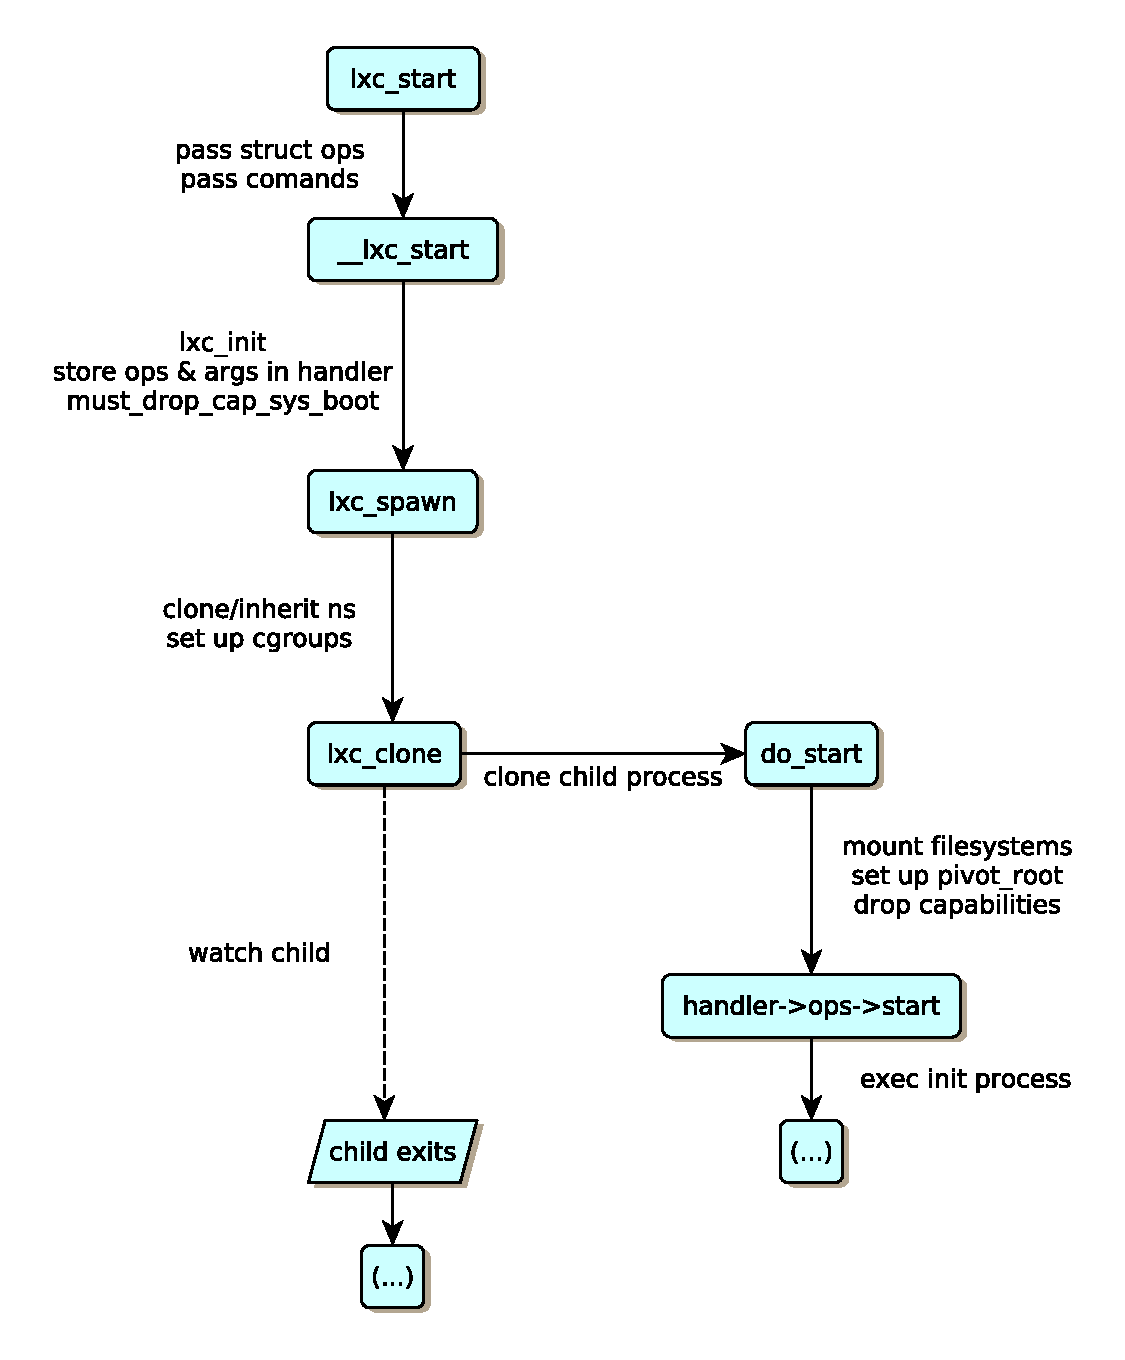
\includegraphics[width=300pt]{fig/figure_1.eps}
  \caption{start flowchart}
  \label{figure_1}
\end{center}
\end{figure}

\section{Capability dropping}\label{caps}

There are two types of users on a linux system: the root user who is basically allowed to do everything and the normal user 
who is not capable of performing any privileged operation. Kernel capabilities are a feature which allow a more distinct way of handling
permissions. In general the procedure is to start a program with root permissions and then dropping capabilities from the prevailing full set.
Any child process spawned will inherit this capability subset.
In some situations it might be more suitable to grant just a few capabilities while dropping the others, or maybe a program wants to do
privileged operations before handing the control over to some unstrustworthy program (which is the case with \textit{lxc}). Note
that unless CAP\_SETPCAP is dropped the program can regrant itself any capability\cite{kernelcaps}.
As mentioned before lxc does not drop its capabilities immediately. The start processes as follows in a stripped down version (see figure \ref{figure_1}):\\
Note that the nodes represent a ``step into'' exept for \textit{lxc\_clone --> child exits} which is a ``step over'' and -- as the parent is
irrelevant at this point for showing how capabilities are dropped -- does not point to another function but rather to a certain state.\\
In \texttt{\_\_lxc\_start} (start.c) the container first executes \texttt{lxc\_init} which mainly loads the seccomp policies (see chapter \ref{seccomp}),
sets the state to ``STARTING'' and environment variables for a pre-setup hook script. On return a \textit{handler} struct is handed to
\texttt{\_\_lxc\_start} which then adds the struct ops containing function references for later use and some commands given be the
initial caller (the first argument must be something like \texttt{/sbin/init}) to execute after lxc is done setting everything up for
the actual init process of the container.
Slightly afterwards \texttt{lxc\_spawn} is executed which then sets up cgroups according to the config specifications,
clones or inherits namespaces and creates a new process through \texttt{lxc\_clone}. This child process in turn executes \texttt{do\_start} which
mounts the filesystems accordingly and ultimately drops the privileges. After that it replaces itself with the init process of
the container through the \texttt{exec()} system call. The parent process waits for the child to complete its startup process and determines
if it simply exited or was signaled because it tried to do a reboot.\\
I have written a minimal c-program to test for capabilities inside the container which prints out every single one with
its label followed by the effective value, \texttt{1} for set \texttt{0} for unset. The code makes use of the shared library
\texttt{libcap.so.2}, so when running inside a container this must be present or else the test will fail.

\section{Mountpoints}

The only mounted filesystem besides the root filesystem is \texttt{/proc}. \texttt{/proc} is crucial for the execution environment because many
different programs rely on it to store and access process information. However while running the test-c-programs no error due
to \texttt{/proc} not being mounted could be detected.\\
The \texttt{/sys} filesystem contains amongst other things pseudofiles for accessing the machine hardware. As untrustworthy programs
having access to hardware settings is highly undesired, the safest yet most radical solution is not to mount \texttt{/sys}.

\section{Seccomp policies}\label{seccomp}

\textit{Seccomp policies} are a rather low level feature. They depend on system specific information such
as the architecture (x64 or x86). Essentially they are currently used by \textit{lxc} to blacklist some unsafe system calls that aim on
modifying the currently running kernel.
\chapter{Lxc issues}

\section{Lxc-python api and threads}

In general c-code is not thread safe, so when executing a c-function through python the default
behaviour of the python interpreter is to block all other running threads until said function returns\cite{gil}.\\
When executing the attach\_wait function all threads would be blocked until it returned. Unfortunately
this made it impossible to stop the container through a timer thread atfer a certain amount of time had
passed (not to speak of running more than one container simultaneously).\\
However there are macros defined in python.h which are able to tell python to temporarily allow threads.
Turning in this patch\cite{bugreport} resolved the issue.


%%%%%%%%%%%%%%%%%%%%%%%%%%%%%%%%%%%%%%%%%%%%%%
%%    End of the main document              %%
%%%%%%%%%%%%%%%%%%%%%%%%%%%%%%%%%%%%%%%%%%%%%%

\backmatter

\bibliographystyle{alphadin} %% german output

\bibliography{sources}

\printindex

\chapter*{Ehrenwörtliche Erklärung}

Hiermit versichere ich, die vorliegende Bachelorarbeit selbstständig 
verfasst und keine anderen als die angegebenen Quellen und Hilfsmittel
benutzt zu haben.
Alle Stellen, die aus den Quellen entnommen
wurden, sind als solche kenntlich gemacht worden. Diese Arbeit hat in
gleicher oder ähnlicher Form noch keiner Prüfungsbehörde vorgelegen.

\vspace{3cm}

\noindent Düsseldorf, 14.Dezember 2004 \hfill Vorname Nachname


\cleardoublepage

\chapter*{}
\thispagestyle{empty}

\begin{center}
  \vspace{-3cm}
  \fbox{\parbox[c][12cm][c]{12cm}{\centering Hier die H\"ulle\\[1cm]mit der CD/DVD einkleben}}
\end{center}

\vfill

\textbf{Diese CD enthält:}
\begin{itemize}
 \item eine \emph{pdf}-Version der vorliegenden Bachelorarbeit
 \item die \LaTeX- und Grafik-Quelldateien der vorliegenden Bachelorarbeit samt aller verwendeten Skripte
 \item die Quelldateien der im Rahmen der Bachelorarbeit erstellten Software \texttt{lxc\_daemon}
 \item die Quelldateien der im Rahmen der Bachelorarbeit erstellten Test-C-Programme
 \item die Websites der verwendeten Internetquellen
\end{itemize}


\end{document}

